\begin{figure*}
  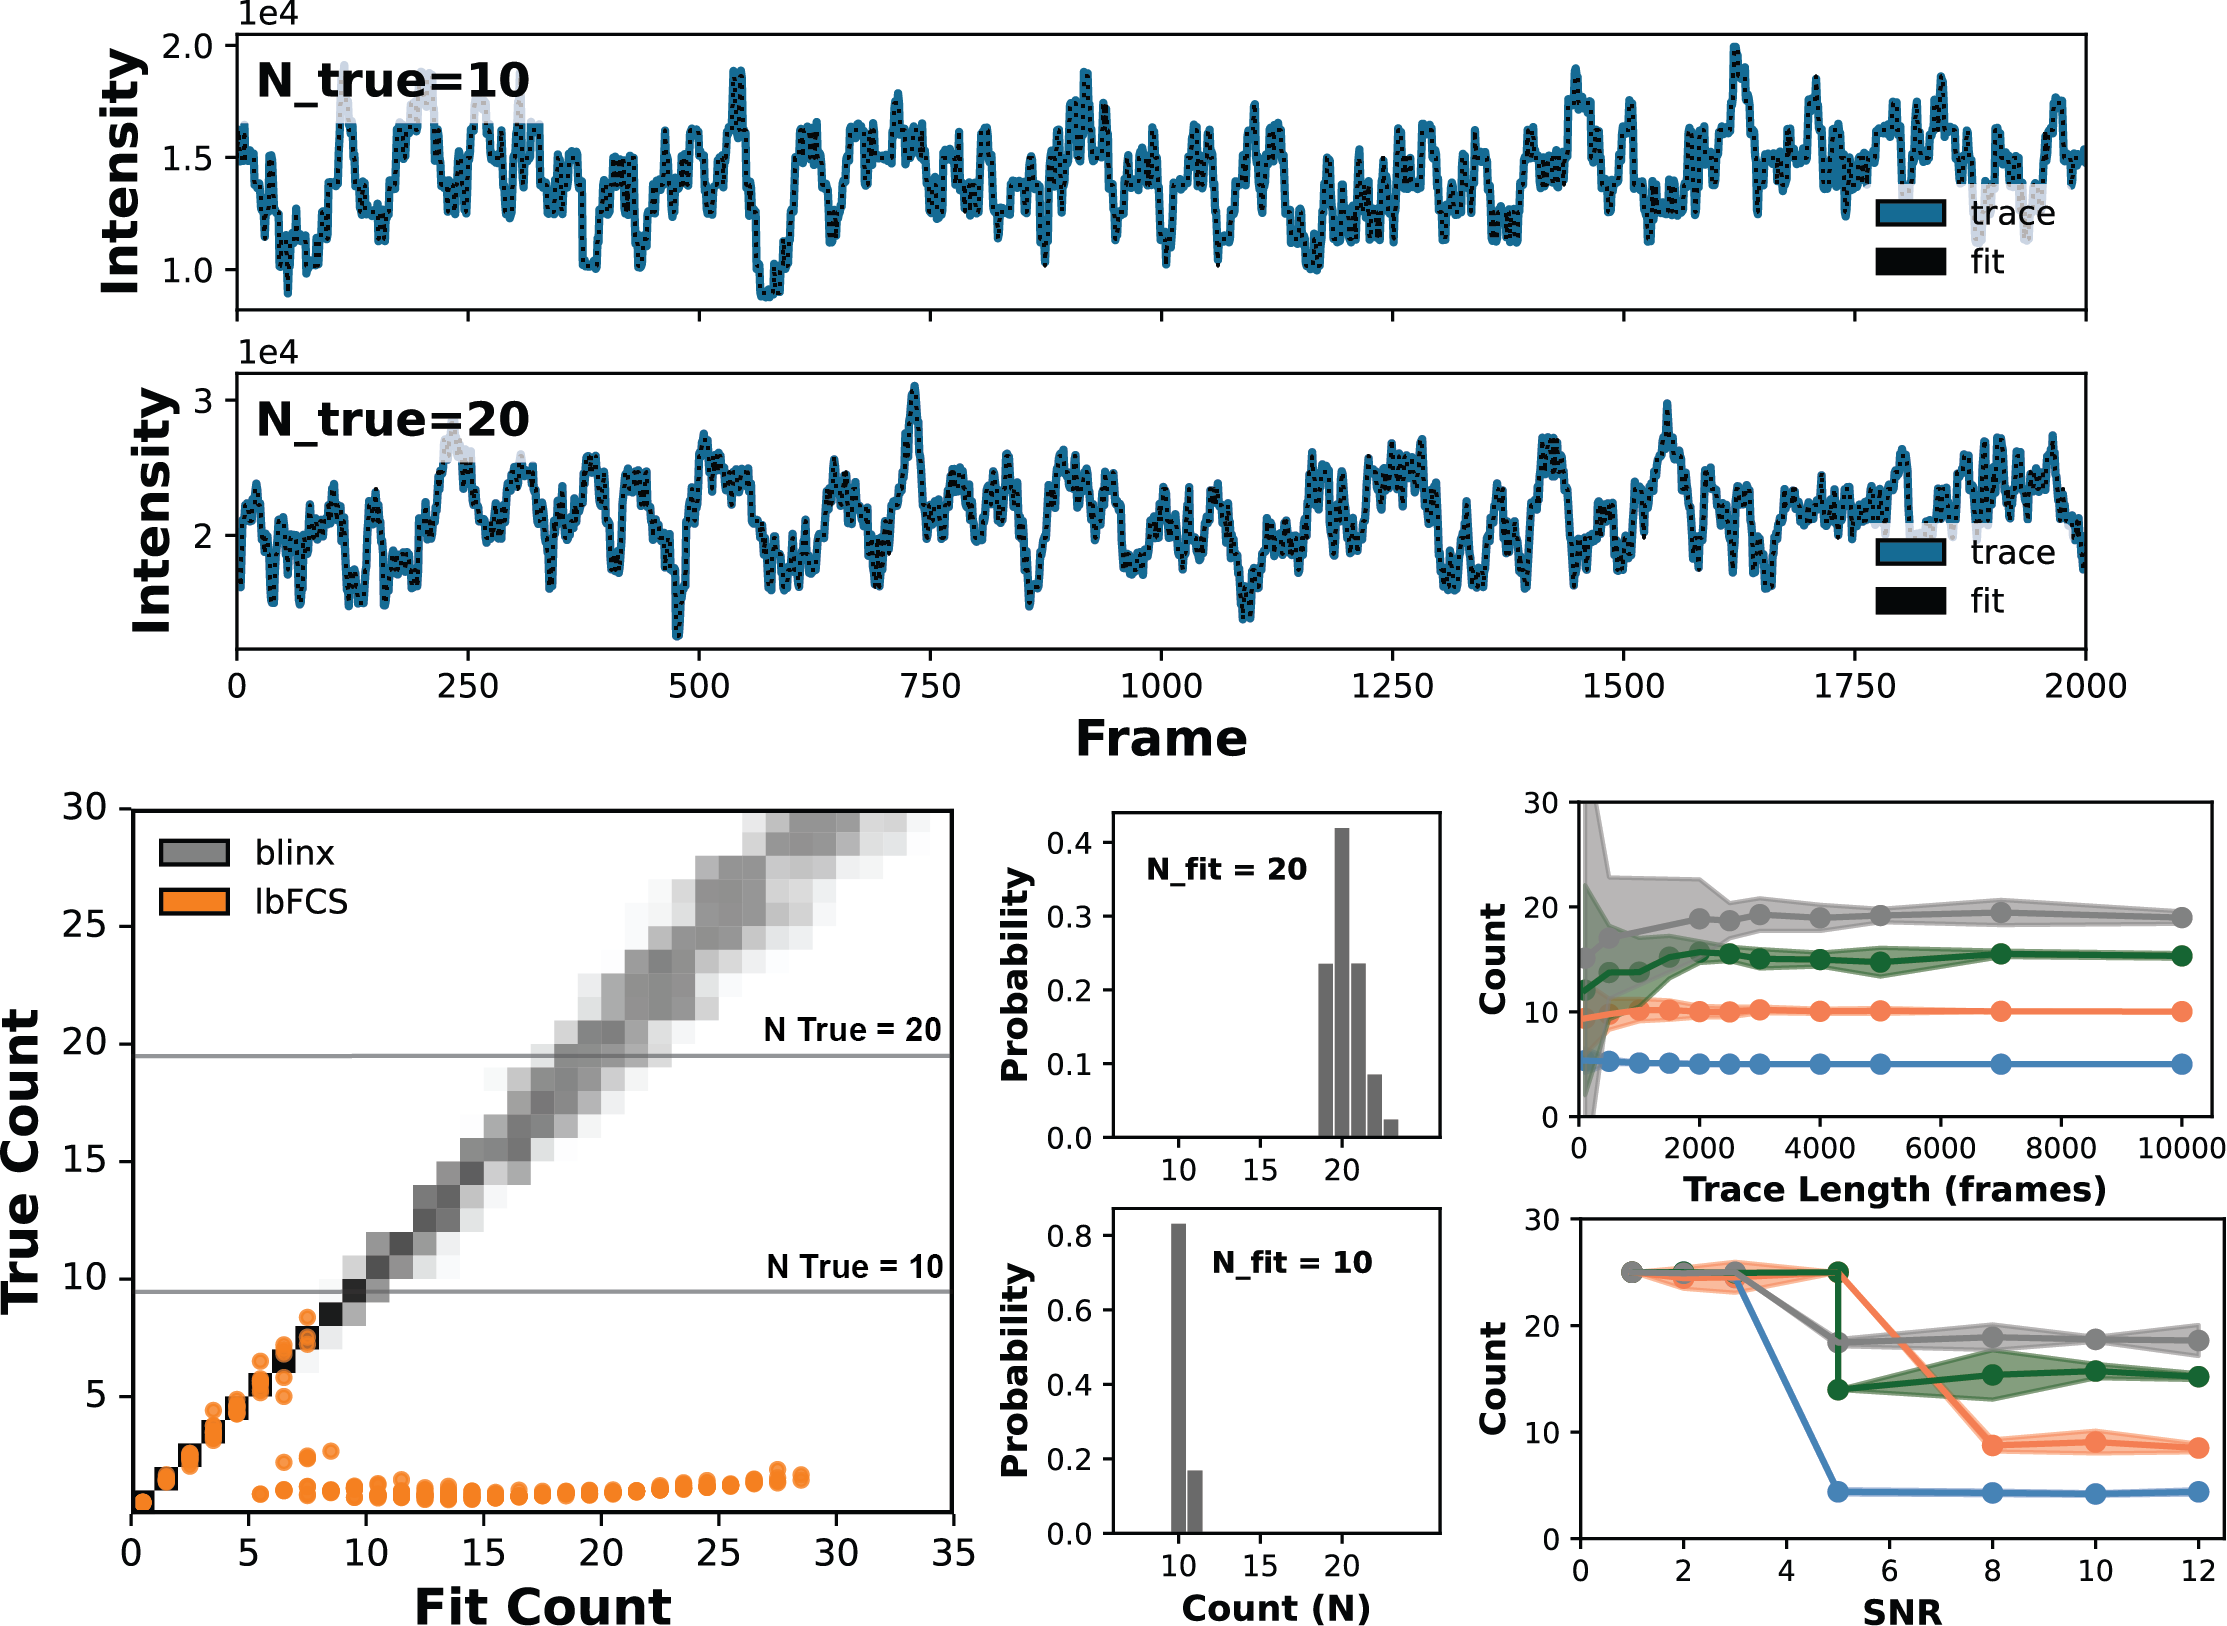
\includegraphics[width=\linewidth]{figures/placeholders/figure_2_simulated_counting.png}
  \caption{A) Trace simulated from 10 emitters, and the posterior distribution estimated by blinx B) simulated from 20 emitters
  C) The blinx posterior is able to accurately estimate significantly higher molecular counts than the current state of the art, lbFCS
  D) As trace length increases, the variance of the blinx posterior decreases E) As the signal to noise ratio increases the variance of 
  the blinx posterior decreases. }
  \label{fig:method:overview}
\end{figure*}
